\documentclass[10pt,aspectratio=169]{beamer}

\usetheme{metropolis}
\usepackage{booktabs}
\usepackage{amsmath}
\usepackage{xcolor}
\usepackage{graphicx}
\usepackage{tikz}
\usetikzlibrary{arrows.meta, positioning, fit, backgrounds, shapes.geometric}

\definecolor{riskon}{HTML}{4F7A4A}
\definecolor{riskoff}{HTML}{B23A3A}
\definecolor{accent}{HTML}{E8743B}
\definecolor{slate}{HTML}{3C4A5A}

% ---- shared TikZ styles -------------------------------------------------
\tikzset{
	stage/.style={draw=accent!75, line width=0.8pt, rounded corners=3pt,
		fill=accent!8, text width=2.7cm, minimum height=1.7cm,
		align=center, inner sep=4pt, font=\footnotesize},
	chip/.style={draw=slate!60, line width=0.7pt, rounded corners=2pt,
		fill=slate!6, align=center, inner sep=4pt, font=\scriptsize},
	arr/.style={-{Stealth[length=3mm]}, line width=1pt, accent!85},
}

\newcommand{\metriccard}[3]{%
	\begin{minipage}[t]{0.23\textwidth}
		\textcolor{accent}{\scriptsize\textbf{#1}}\\[-0.1em]
		{\Large\textbf{#2}}\\[-0.2em]
		{\scriptsize #3}
	\end{minipage}%
}

\title{Detecting Abnormal Markets}
\subtitle{Early Warning Systems with Deep \& Classical Anomaly Detection}
\date{\today}
\author[Peng Rao et al.]{\texorpdfstring{\scriptsize Peng Rao, Maxime d'Aviau de Ternay, Qiao Zhaochen,\\ Shourya Vashistha, Arnau Nomen}{Peng Rao et al.}}
\institute{Politecnico di Milano}

\begin{document}

\maketitle

% =========================================================================
\begin{frame}{Why this matters}
	\begin{columns}[T,onlytextwidth]
		\column{0.52\textwidth}
		\textbf{Crashes are rare but decisive} -- 1929, 2000, 2008, 2020 \dots
		\vspace{0.5em}

		A handful of days drives a lifetime of returns. \\
		\textbf{Buy-and-hold S\&P 500, 1927--2015:}
		\begin{center}
			\small
			\begin{tabular}{lr}
				\toprule
				Strategy               & Growth of \$1      \\
				\midrule
				Stay invested          & \$115.40           \\
				Miss the 10 worst days & \$362.01           \\
				Miss the 10 best days  & \phantom{0}\$38.28 \\
				\bottomrule
			\end{tabular}
		\end{center}

		\column{0.44\textwidth}
		\begin{alertblock}{Tail events cluster}
			The frequency and cross-asset correlation of simultaneous heavy
			losses keep rising. \\[0.4em]
			Diversification fails exactly when you need it most -- so we need a
			signal that fires \emph{before} the drawdown compounds.
		\end{alertblock}
	\end{columns}
\end{frame}

% =========================================================================
\begin{frame}{The transition we must catch}
	\begin{columns}[T,onlytextwidth]
		\column{0.48\textwidth}
		\begin{block}{\color{riskon}\textbf{Risk-on}}
			\small Confidence. Equities, credit, EM, commodities bid up.
			Volatility low, spreads tight, capital chases growth.
		\end{block}
		\column{0.48\textwidth}
		\begin{block}{\color{riskoff}\textbf{Risk-off}}
			\small Fear. Flight to cash, short govies, gold, CHF, JPY.
			Volatility spikes, correlations surge -- systemic risk.
		\end{block}
	\end{columns}
	\vspace{0.5em}
	\begin{center}
		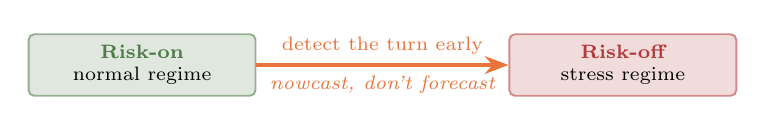
\begin{tikzpicture}[font=\footnotesize]
			\node[chip, fill=riskon!18, draw=riskon!60, text width=2.6cm] (on) {\textbf{\color{riskon}Risk-on}\\\scriptsize normal regime};
			\node[chip, fill=riskoff!18, draw=riskoff!60, text width=2.6cm, right=3.2cm of on] (off) {\textbf{\color{riskoff}Risk-off}\\\scriptsize stress regime};
			\draw[-{Stealth[length=3mm]}, line width=1.2pt, accent]
			(on) -- node[above,font=\scriptsize]{detect the turn early}
			node[below,font=\scriptsize\itshape]{nowcast, don't forecast} (off);
		\end{tikzpicture}
	\end{center}
	\centering\small
	We do not predict \emph{which} crash. We flag, in real time, that this week is
	\textbf{``not normal''} -- a 2008-style and a 2020-style stress both qualify.
\end{frame}

% =========================================================================
\begin{frame}{Pipeline: from raw prices to a risk-off flag}
	\vspace{0.2em}
	\begin{center}
		\resizebox{\textwidth}{!}{%
			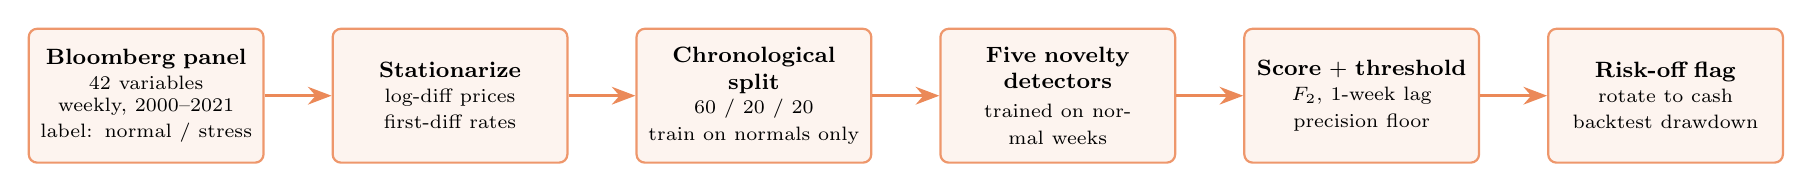
\begin{tikzpicture}
				\node[stage] (data) {\textbf{Bloomberg panel}\\[1pt]\scriptsize 42 variables\\weekly, 2000--2021\\label: normal / stress};
				\node[stage, right=0.85cm of data] (stat) {\textbf{Stationarize}\\[1pt]\scriptsize log-diff prices\\first-diff rates};
				\node[stage, right=0.85cm of stat] (split) {\textbf{Chronological split}\\[1pt]\scriptsize 60 / 20 / 20\\train on normals only};
				\node[stage, right=0.85cm of split] (det) {\textbf{Five novelty\\detectors}\\[1pt]\scriptsize trained on normal weeks};
				\node[stage, right=0.85cm of det] (thr) {\textbf{Score $+$ threshold}\\[1pt]\scriptsize $F_2$, 1-week lag\\precision floor};
				\node[stage, right=0.85cm of thr] (bt) {\textbf{Risk-off flag}\\[1pt]\scriptsize rotate to cash\\backtest drawdown};
				\foreach \a/\b in {data/stat, stat/split, split/det, det/thr, thr/bt}
				\draw[arr] (\a) -- (\b);
			\end{tikzpicture}}
	\end{center}
	\vspace{0.4em}
	\small
	\begin{itemize}
		\item Treat \textbf{normal markets} as the inlier distribution; train on normals
		      only and flag high anomaly scores -- no need to label crisis types ex ante.
		\item Deployment: a flag rotates into cash / short govies / gold. User: CIO,
		      risk officer, wealth manager. \textbf{Goal = cut drawdown}, not chase alpha.
	\end{itemize}
\end{frame}

% =========================================================================
\begin{frame}{Data: stress clusters around drawdowns}
	\begin{columns}[T,onlytextwidth]
		\column{0.56\textwidth}
		\centering
		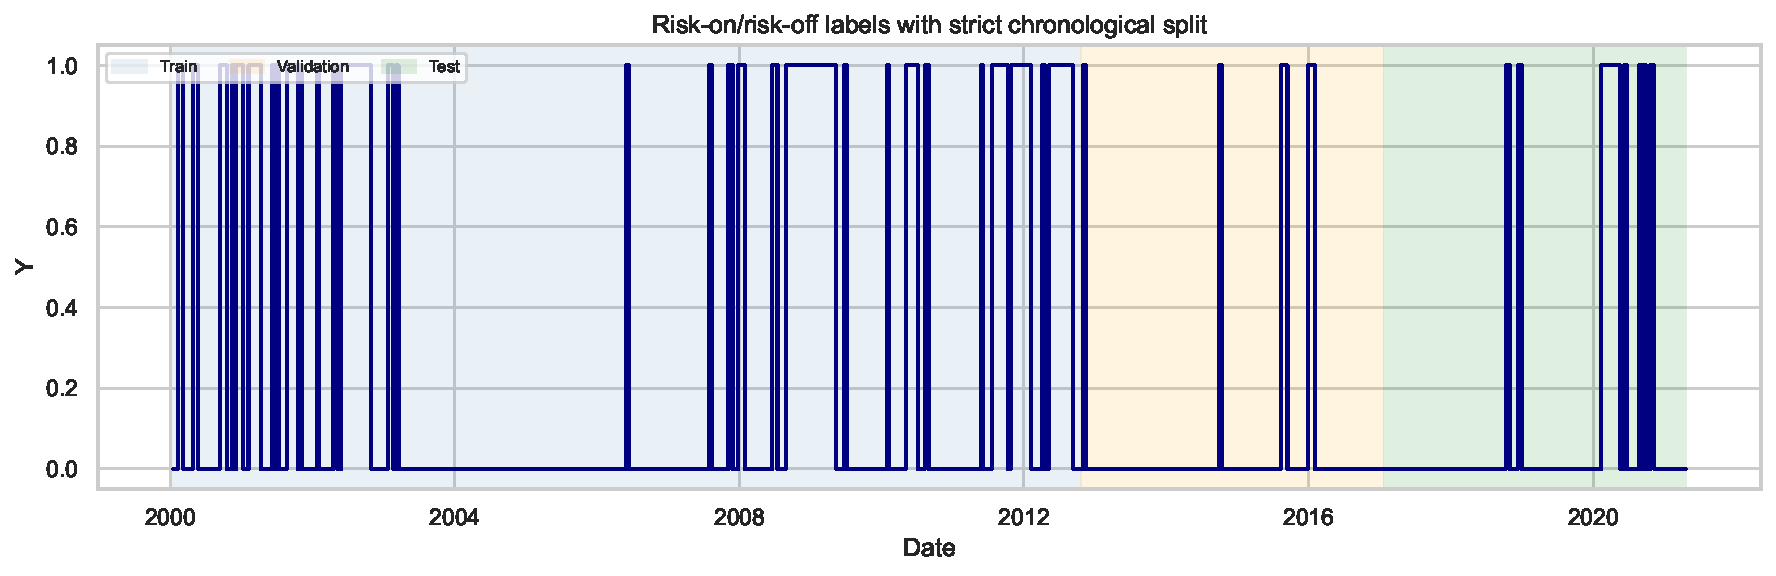
\includegraphics[width=\textwidth,height=0.62\textheight,keepaspectratio]{figures/01_stationary_anomaly_labels.pdf}\\
		{\scriptsize US equity (MXUS) with stress weeks shaded}
		\column{0.42\textwidth}
		\centering
		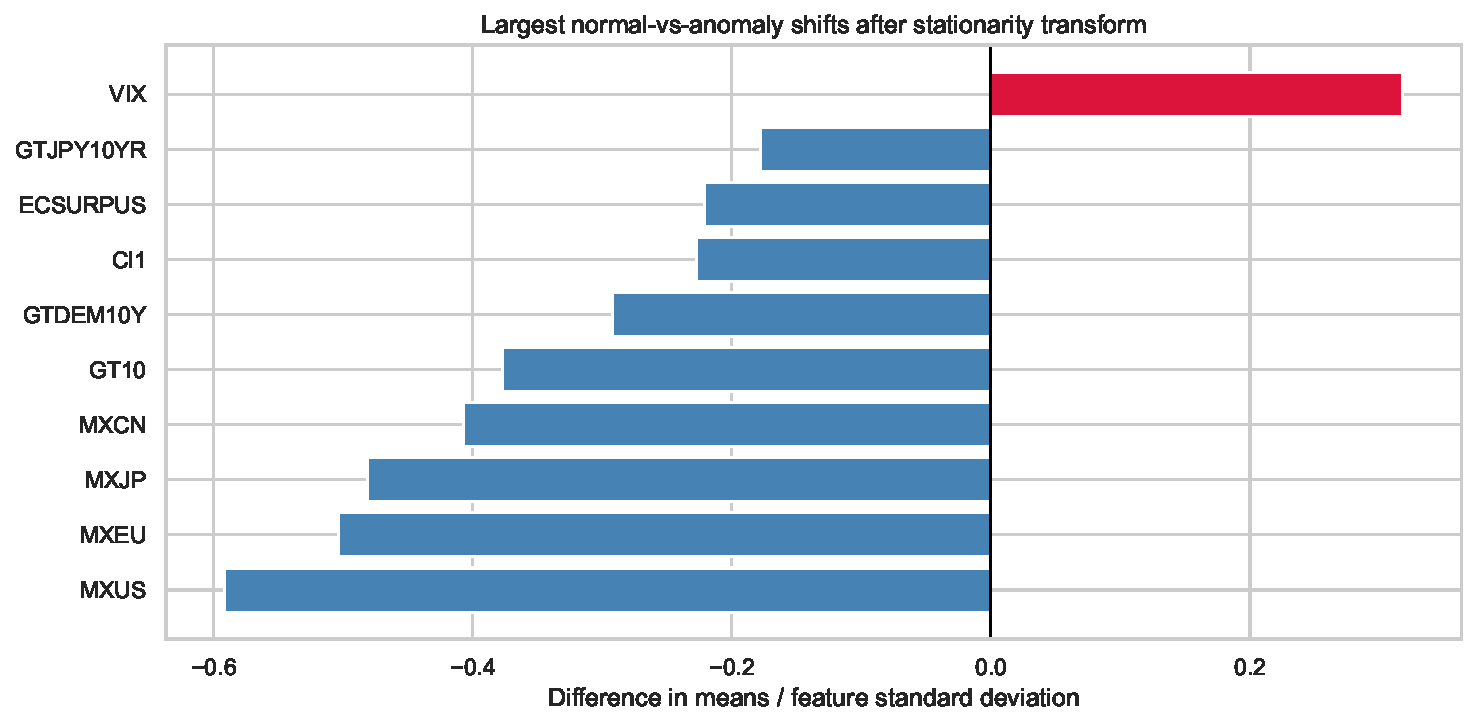
\includegraphics[width=\textwidth,height=0.62\textheight,keepaspectratio]{figures/03_eda_largest_feature_shifts.pdf}\\
		{\scriptsize Largest standardized mean shifts, normal vs.\ stress}
	\end{columns}
	\vspace{0.3em}
	\footnotesize
	1110 weekly observations $\times$ 42 features; \textbf{21\%} of weeks labelled
	abnormal. Stress weeks line up with equity selloffs and load on equity returns
	(MXUS, MXEU, MXJP) and the VIX -- the signal is real and economically sensible.
\end{frame}

% =========================================================================
\begin{frame}{Five detectors, two families}
	\centering
	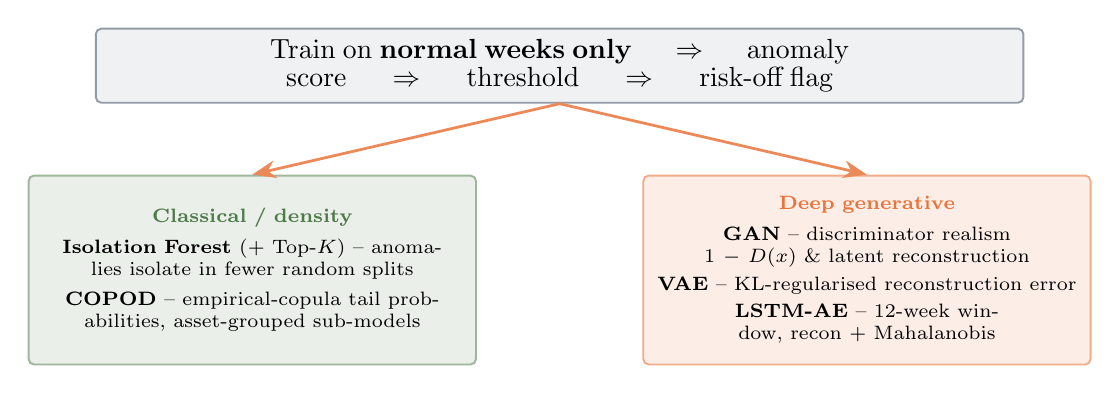
\begin{tikzpicture}[font=\scriptsize]
		\node[chip, fill=slate!8, draw=slate!55, text width=11.5cm, minimum height=0.8cm]
		(root) {\normalsize Train on \textbf{normal weeks only} $\;\Rightarrow\;$ anomaly score $\;\Rightarrow\;$ threshold $\;\Rightarrow\;$ risk-off flag};

		\node[chip, fill=riskon!12, draw=riskon!55, text width=5.4cm, minimum height=2.4cm,
			below left=0.9cm and -2.0cm of root, anchor=north] (cls)
		{\textbf{\color{riskon}Classical / density}\\[3pt]
		\textbf{Isolation Forest} ($+$ Top-$K$) -- anomalies isolate in fewer random splits\\[3pt]
		\textbf{COPOD} -- empirical-copula tail probabilities, asset-grouped sub-models};

		\node[chip, fill=accent!12, draw=accent!60, text width=5.4cm, minimum height=2.4cm,
			below right=0.9cm and -2.0cm of root, anchor=north] (dl)
		{\textbf{\color{accent}Deep generative}\\[3pt]
		\textbf{GAN} -- discriminator realism $1-D(x)$ \& latent reconstruction\\[2pt]
		\textbf{VAE} -- KL-regularised reconstruction error\\[2pt]
		\textbf{LSTM-AE} -- 12-week window, recon $+$ Mahalanobis};

		\draw[arr] (root.south) -- (cls.north);
		\draw[arr] (root.south) -- (dl.north);
	\end{tikzpicture}
	\vspace{0.4em}

	\footnotesize One shared objective ($F_2$) tunes every threshold $\Rightarrow$ comparable operating points across all five.
\end{frame}

% =========================================================================
\begin{frame}{Honest evaluation: no look-ahead}
	\centering
	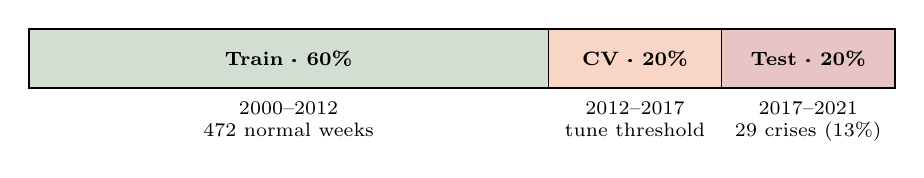
\begin{tikzpicture}[font=\scriptsize]
		\fill[riskon!25] (0,0) rectangle (6.6,0.75);
		\fill[accent!30] (6.6,0) rectangle (8.8,0.75);
		\fill[riskoff!30] (8.8,0) rectangle (11,0.75);
		\draw[line width=0.8pt] (0,0) rectangle (11,0.75);
		\draw (6.6,0)--(6.6,0.75); \draw (8.8,0)--(8.8,0.75);
		\node at (3.3,0.375){\textbf{Train · 60\%}};
		\node at (7.7,0.375){\textbf{CV · 20\%}};
		\node at (9.9,0.375){\textbf{Test · 20\%}};
		\node[below, align=center] at (3.3,-0.05){2000--2012\\472 normal weeks};
		\node[below, align=center] at (7.7,-0.05){2012--2017\\tune threshold};
		\node[below, align=center] at (9.9,-0.05){2017--2021\\29 crises (13\%)};
	\end{tikzpicture}
	\vspace{0.8em}

	\begin{columns}[T,onlytextwidth]
		\column{0.5\textwidth}
		\textbf{Strict chronological split}
		\begin{itemize}\small
			\item Fit on the \emph{past} only -- faithful to live deployment.
			\item Threshold: all five maximise $F_2$ ($\beta=2.0$, recall weighted 4$\times$),
			      subject to a precision floor.
			\item Backtest acts on the signal with a \textbf{1-week lag} -- no same-week look-ahead.
		\end{itemize}
		\column{0.5\textwidth}
		\textbf{Metrics for the risk officer}
		\begin{itemize}\small
			\item \textbf{Recall / FNR} -- a missed crisis is the costly failure.
			\item \textbf{PR-AUC} -- honest under heavy class imbalance.
			\item Precision, F1, ROC-AUC reported for completeness.
		\end{itemize}
	\end{columns}
	\vspace{0.2em}
	\centering\footnotesize
	\textcolor{riskoff}{No shuffling, no leakage} -- numbers are deliberately conservative and deployable.
\end{frame}

% =========================================================================
% PART 1 -- Isolation Forest
% =========================================================================
\begin{frame}{Part 1 $\cdot$ Isolation Forest: the warning signal in action}

    \centering

    % --- Top graph ---
    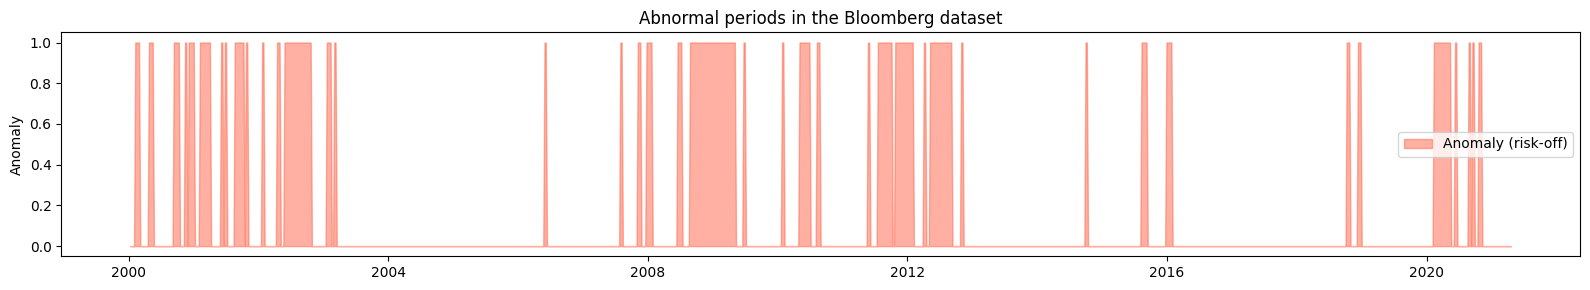
\includegraphics[
        width=0.88\textwidth,
        height=0.34\textheight,
        keepaspectratio
    ]{figures/abnormal_periods.png}

    \vspace{0.1cm}

    {\scriptsize Abnormal periods over time}

    \vspace{0.35cm}

    % --- Bottom part ---
    \begin{columns}[T,onlytextwidth]

        % Left: bullet points
        \begin{column}{0.52\textwidth}
            \begin{itemize}
                \footnotesize
                \item Weekly data collection.
                \item Binary target variable: $Y = 1$ for abnormal periods and $Y = 0$ otherwise.
                \item Strong class imbalance: anomalies are rare but critical to detect.
            \end{itemize}
        \end{column}

        % Right: second graph
        \begin{column}{0.65\textwidth}
            \centering
            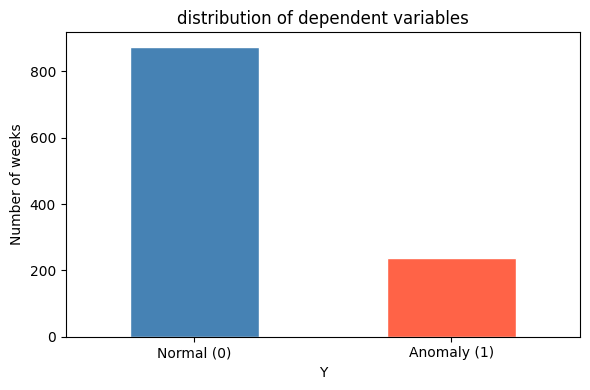
\includegraphics[
                width=\textwidth,
                height=0.33\textheight,
                keepaspectratio
            ]{figures/class_distribution.png}

            \vspace{0.05cm}

            {\scriptsize Class distribution}
        \end{column}

    \end{columns}

\end{frame}
% =========================================================================

\begin{frame}{2. Isolation Forest: Feature engineering}

\small

Feature engineering consists in creating new variables from the original financial time series.
The goal is to extract more informative signals for anomaly detection.

\vspace{0.35cm}

\begin{columns}[T,onlytextwidth]

% Left column
\begin{column}{0.48\textwidth}
{\bfseries Why create new features?}

\vspace{0.15cm}

\begin{itemize}
    \footnotesize

    \item New variables help capture hidden market dynamics.
    \item They make the model more sensitive to abnormal periods.
\end{itemize}

\vspace{0.25cm}

{\bfseries Examples of engineered features}

\vspace{0.15cm}

\begin{itemize}
    \footnotesize
    \item \textbf{Volatility:} measures the instability of a variable.
    \item \textbf{Momentum:} captures short-term upward or downward trends.
    \item \textbf{Drawdown:} detects strong decreases from previous peaks.
\end{itemize}

\end{column}

% Right column
\begin{column}{0.48\textwidth}
{\bfseries What does it improve?}

\vspace{0.15cm}

\begin{itemize}
    \footnotesize
    \item Volatility features help identify periods of financial stress.
    \item Momentum features capture changes in market direction.
    \item Drawdown features highlight sudden losses or regime shifts.
\end{itemize}

\vspace{0.25cm}

{\bfseries Feature selection}

\vspace{0.15cm}

\begin{itemize}
    \footnotesize
    \item We keep variables that bring useful information.
    \item Highly redundant variables are removed.
    \item Selected features have low covariance or weak dependence, reducing overlap between signals.
\end{itemize}

\end{column}

\end{columns}

\vspace{0.25cm}

\begin{center}
\footnotesize
\textit{Feature engineering helps the Isolation Forest detect abnormal patterns that are not directly visible in raw data.}
\end{center}

\end{frame}
% =========================================================================

\begin{frame}{3. Isolation Forest model}

\centering

% --- Large graph on top ---
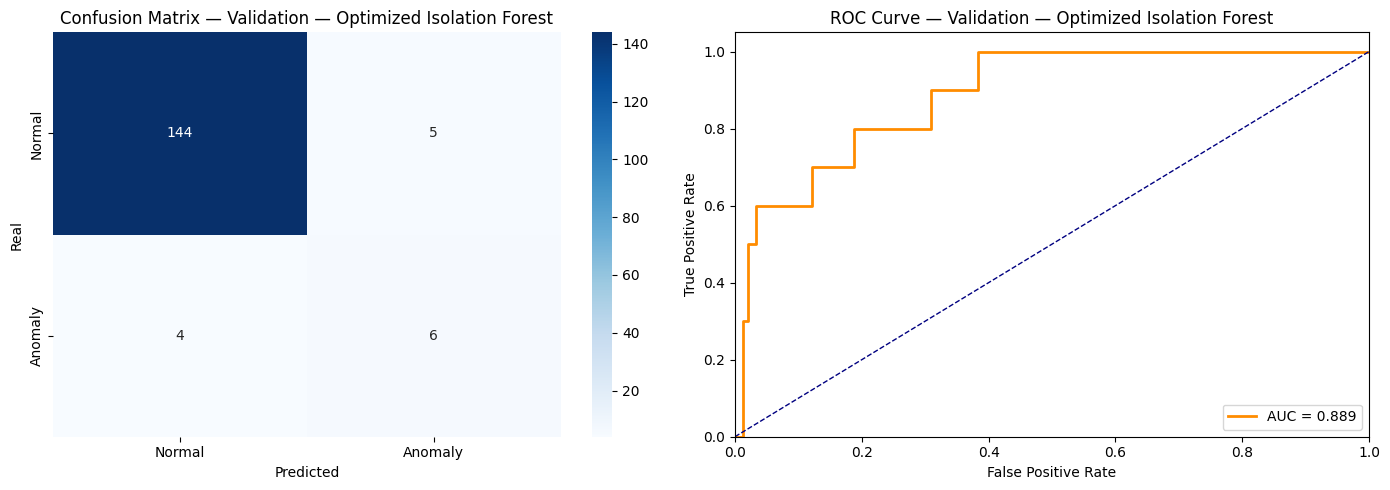
\includegraphics[
    width=0.95\textwidth,
    height=0.58\textheight,
    keepaspectratio
]{figures/confusion_roc_test.png}

\vspace{0.25cm}

% --- Short explanations at the bottom ---
\begin{columns}[T,onlytextwidth]

\begin{column}{0.48\textwidth}
{\bfseries Training strategy}

\vspace{0.08cm}

\begin{itemize}
    \footnotesize
    \item Trained on the training set.
    \item Threshold optimized on validation data.
    \item Final evaluation on the test set.
\end{itemize}
\end{column}

\begin{column}{0.48\textwidth}
{\bfseries Main idea}

\vspace{0.05cm}

\begin{itemize}
    \footnotesize
    \item Anomalies are easier to isolate.
    \item Fewer splits indicate suspicious points.
    \item The model outputs an anomaly score.
\end{itemize}
\end{column}

\end{columns}

\end{frame}

% =========================================================================

\begin{frame}{4. Isolation Forest: Temporal visualization of warning signals}

\centering

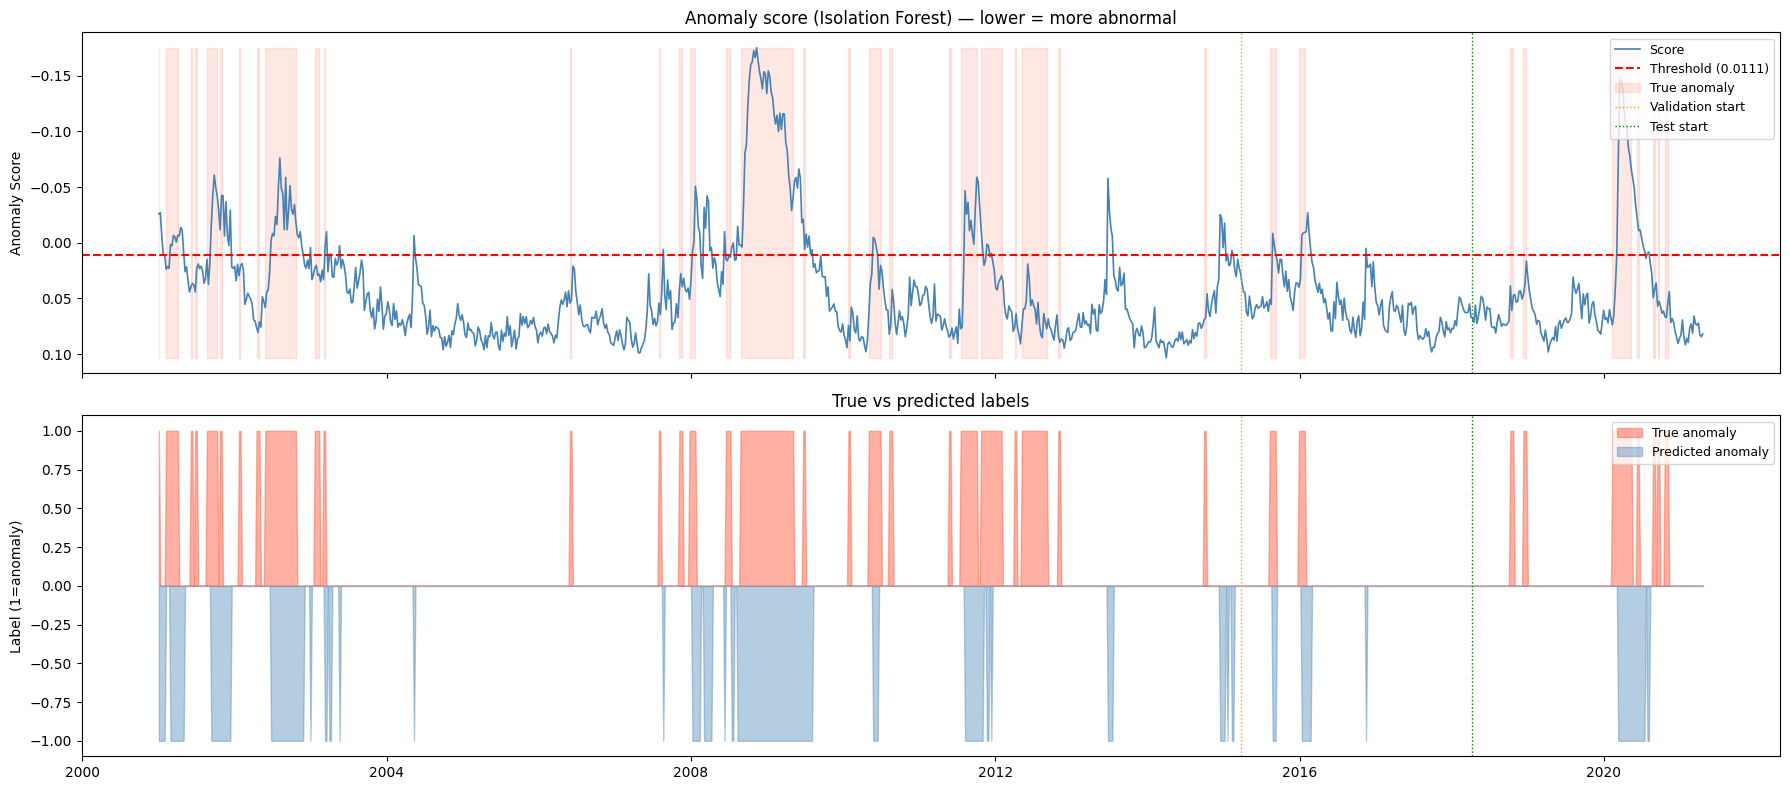
\includegraphics[
    width=0.95\linewidth,
    height=0.80\textheight,
    keepaspectratio
]{figures/signals_backtest.png}

\vspace{0.2cm}

\begin{itemize}
    \footnotesize
    \item Crisis periods are associated with a deterioration of the anomaly score.
    \item The threshold converts a continuous score into an actionable warning signal.
    \item The threshold choice controls the trade-off between detected crises and false alerts.
\end{itemize}

\end{frame}

% =========================================================================

% -----------------------------------------------------------------------------
\begin{frame}{5. Isolation Forest: Interpretation and improvement}

\small

\begin{columns}[T,onlytextwidth]

% Left column: large image
\begin{column}{0.60\textwidth}
    \centering

    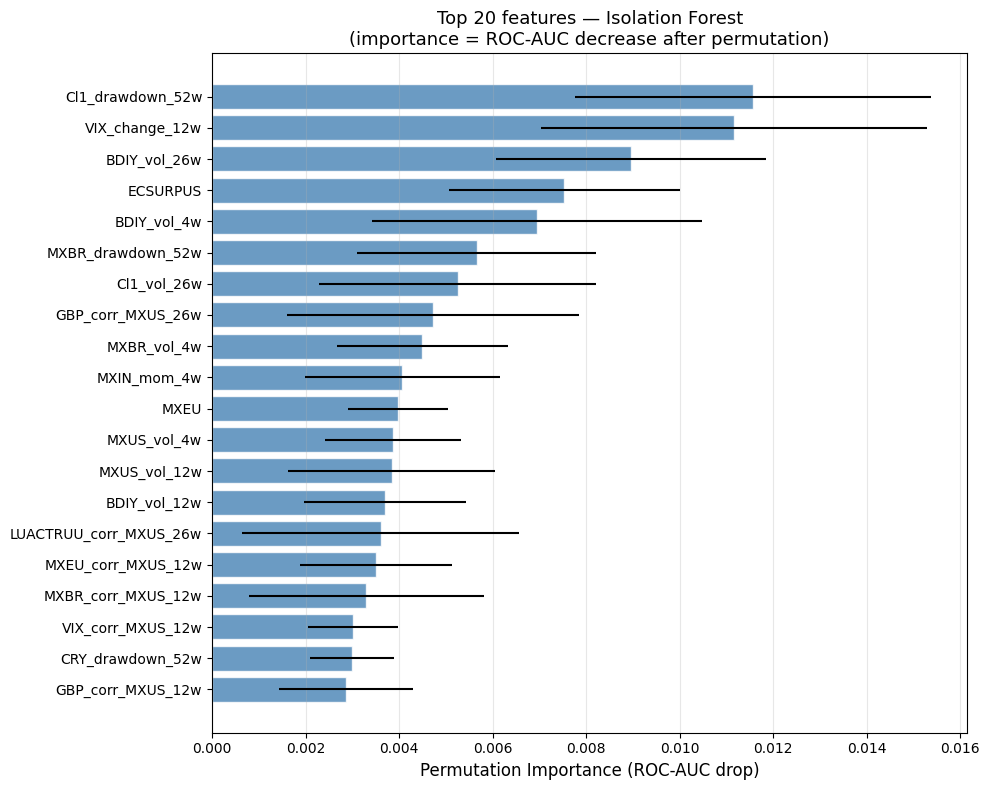
\includegraphics[
        width=\textwidth,
        height=0.9\textheight,
        keepaspectratio
    ]{figures/feature_importance.png}

    \vspace{0.05cm}

    {\scriptsize Feature importance analysis}
\end{column}

% Right column: concise text
\begin{column}{0.38\textwidth}

{\bfseries Key interpretation}

\vspace{0.12cm}

\begin{itemize}
    \footnotesize
    \item The most important features are consistent with financial stress signals.
    \item They include oil, VIX, Baltic Dry Index, macroeconomic surprises and drawdowns.
    \item This improves the interpretability of the anomaly detection model.
\end{itemize}

\vspace{0.25cm}

{\bfseries Top-K variant}

\vspace{0.12cm}

\begin{itemize}
    \footnotesize
    \item More sensitive to anomalies.
    \item Higher crisis detection rate.
    \item Also produces more false alerts.
\end{itemize}

\vspace{0.20cm}

\begin{center}
    \metric{0.76}{test recall Top-K}\\[0.18cm]
    \metric{0.47}{test precision Top-K}\\[0.18cm]
    \metric{0.67}{test $F_2$ Top-K}
\end{center}

\end{column}

\end{columns}

\end{frame}

% =========================================================================
% PART 2 -- COPOD
% =========================================================================
\begin{frame}{Part 2 $\cdot$ COPOD: copula tails, asset-grouped}
	\begin{columns}[c,onlytextwidth]
		\column{0.39\textwidth}
		\centering
		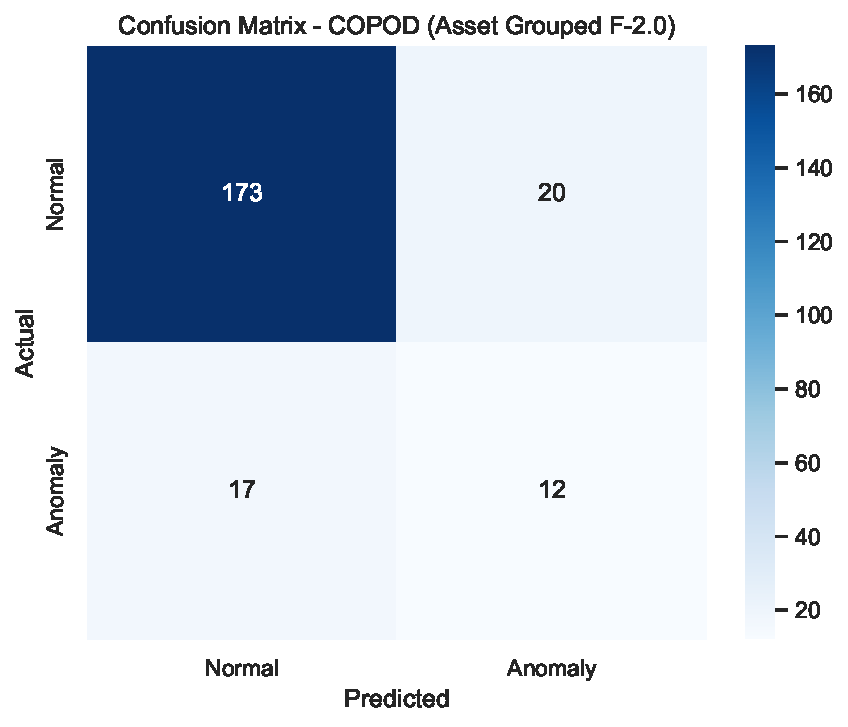
\includegraphics[width=\textwidth,height=0.62\textheight,keepaspectratio]{figures/copod_02_confusion_matrix_copod_asset_grouped_f_2_0.pdf}
		\column{0.59\textwidth}
		\centering
		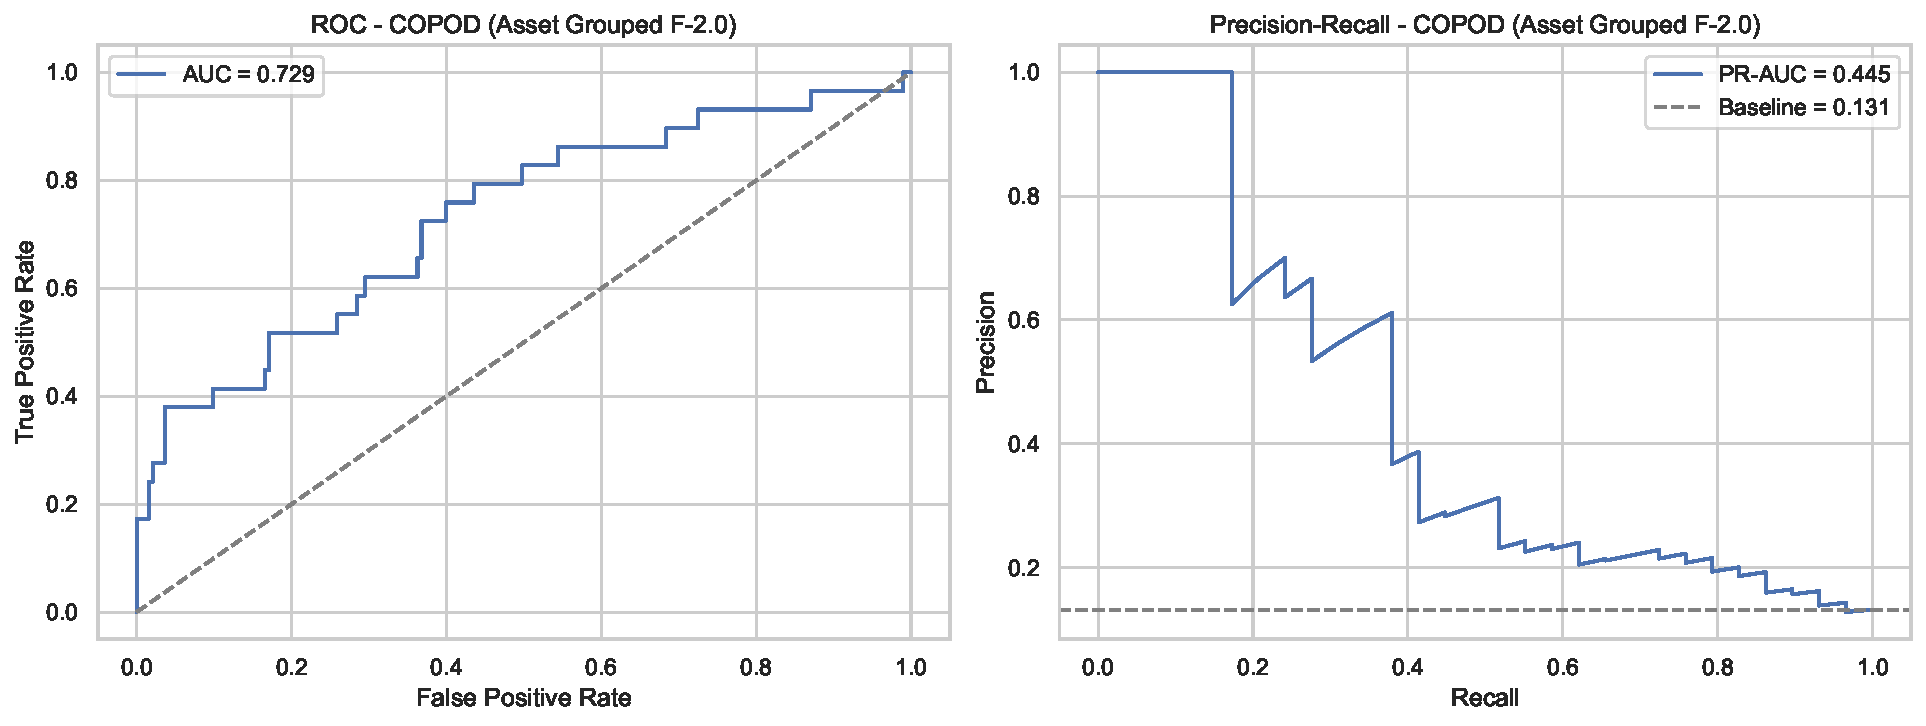
\includegraphics[width=\textwidth,height=0.44\textheight,keepaspectratio]{figures/copod_03_roc_pr_copod_asset_grouped_f_2_0.pdf}

		\vspace{0.3em}
		\footnotesize
		Per-feature \textbf{min(left, right) tail probability}, aggregated as
		$-\tfrac1d\sum\ln(\cdot)$. Four asset families $\to$ sub-COPOD $\to$ meta-COPOD
		avoids \emph{feature dilution}. Test: recall 41\%, PR-AUC 0.45 ($\sim4\times$ baseline).
	\end{columns}
\end{frame}

% =========================================================================
\begin{frame}{Part 2 $\cdot$ COPOD: amber / red operational gates}
	\begin{columns}[c,onlytextwidth]
		\column{0.44\textwidth}
		\centering
		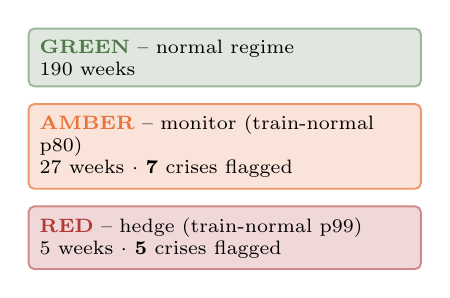
\begin{tikzpicture}[font=\scriptsize]
			\node[chip, fill=riskon!18, draw=riskon!55, text width=4.7cm, align=left] (g)
			{\textbf{\color{riskon}GREEN} -- normal regime\\190 weeks};
			\node[chip, fill=accent!20, draw=accent!75, text width=4.7cm, align=left, below=2mm of g] (a)
			{\textbf{\color{accent}AMBER} -- monitor (train-normal p80)\\27 weeks $\cdot$ \textbf{7} crises flagged};
			\node[chip, fill=riskoff!20, draw=riskoff!60, text width=4.7cm, align=left, below=2mm of a] (r)
			{\textbf{\color{riskoff}RED} -- hedge (train-normal p99)\\5 weeks $\cdot$ \textbf{5} crises flagged};
		\end{tikzpicture}

		\vspace{0.5em}
		\footnotesize \textbf{12/29} crises caught, 17 missed; \textbf{20/20} low-severity
		false alarms parked in the zero-cost amber bucket.
		\column{0.54\textwidth}
		\centering
		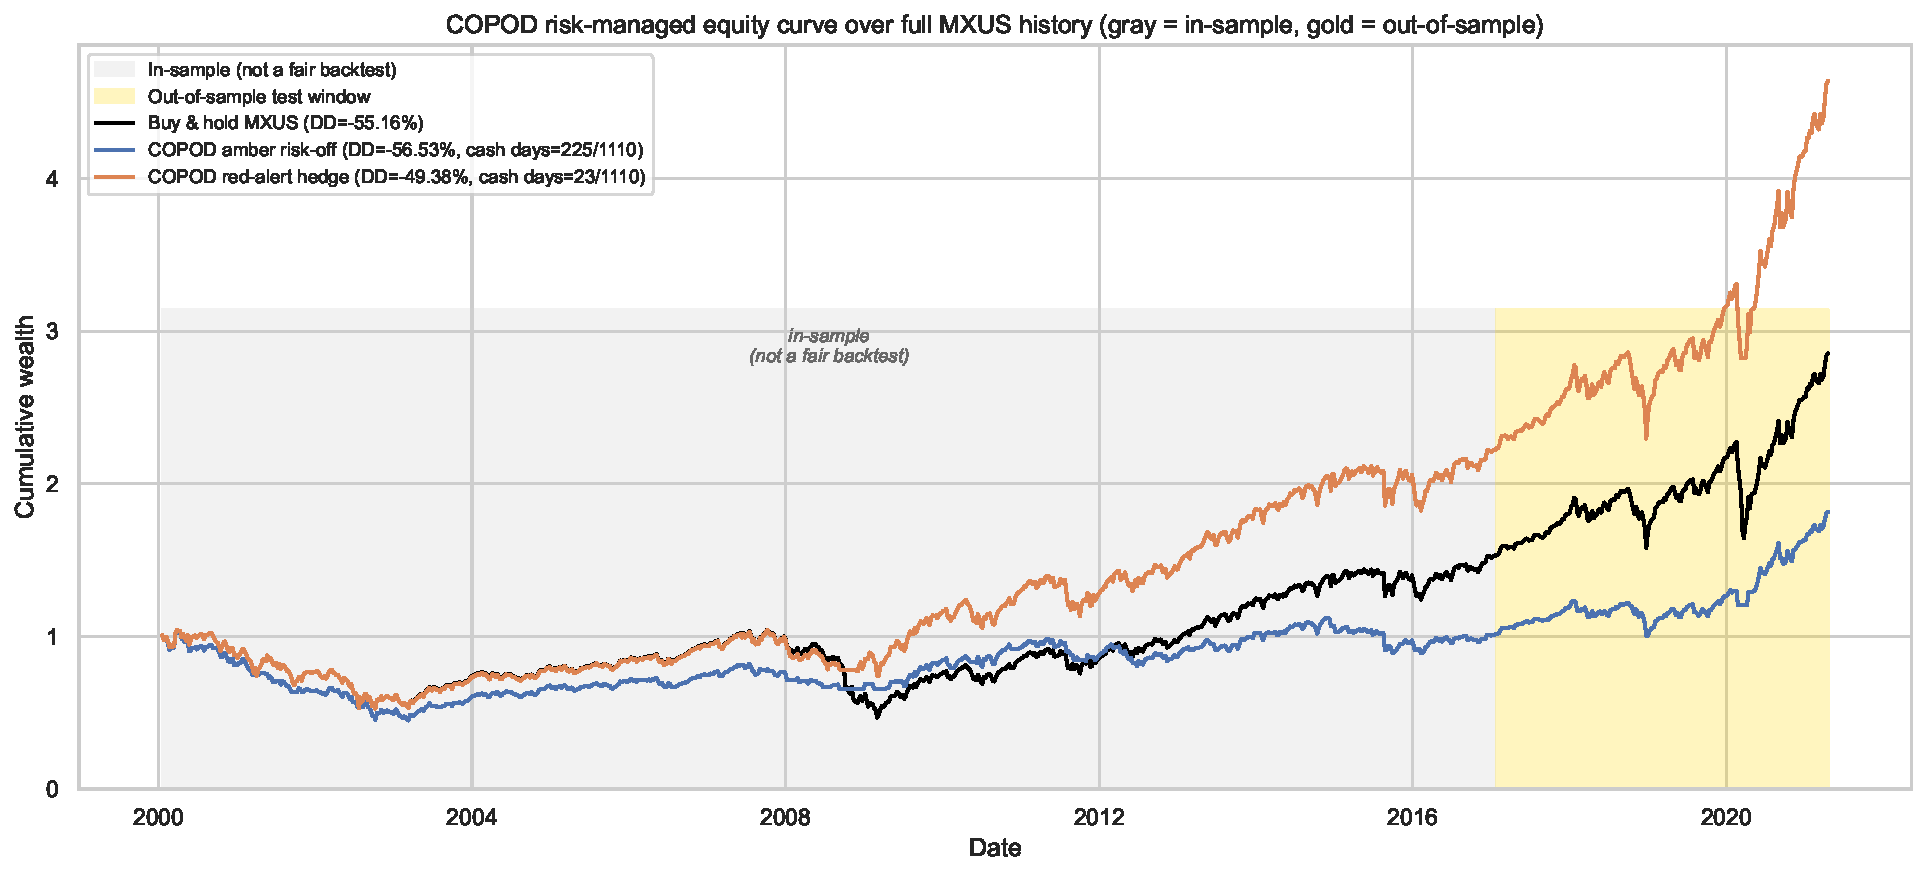
\includegraphics[width=\textwidth,height=0.72\textheight,keepaspectratio]{figures/copod_05_risk_managed_equity_curve.pdf}\\
		{\scriptsize Amber rotates to cash -- out-of-sample wealth 1.80, DD $-18.4\%$.}
	\end{columns}
\end{frame}

\begin{frame}{Cross-model scoreboard (out-of-sample test)}
	\begin{columns}[T,onlytextwidth]
		\column{0.6\textwidth}
		\vspace{0.3em}
		\small
		\setlength{\tabcolsep}{4.5pt}
		\begin{tabular}{lcccc}
			\toprule
			Detector                  & Caught         & Recall          & Prec.           & F2             \\
			\midrule
			Top-$K$ Isolation Forest  & \textbf{24/29} & \textbf{82.8\%} & 58.5\%          & \textbf{0.764} \\
			Optimized Isol.\ Forest   & 14/29          & 48.3\%          & 58.3\%          & 0.500          \\
			COPOD (asset-grouped)     & 12/29          & 41.4\%          & 37.5\%          & 0.405          \\
			VAE reconstruction        & 8/29           & 27.6\%          & \textbf{80.0\%} & 0.317          \\
			LSTM autoencoder          & 8/29           & 27.6\%          & \textbf{80.0\%} & 0.317          \\
			GAN reconstruction        & 8/29           & 27.6\%          & \textbf{80.0\%} & 0.317          \\
			GAN discriminator         & 4/29           & 13.8\%          & 50.0\%          & 0.161          \\
			\bottomrule
		\end{tabular}
		\vspace{0.4em}\\
		{\scriptsize 29 true crises in the held-out 2017--2021 test window.}

		\column{0.38\textwidth}
		\textcolor{accent}{\textbf{The read}}
		\begin{itemize}\small
			\item \textbf{No free lunch}: recall vs.\ precision is a choice, not a ranking.
			\item \textbf{Top-$K$ IF} = recall champion: catches 24 of 29 crises.
			\item \textbf{Deep models} = precision champions: fire rarely, right 80\% of the time.
			\item \textbf{COPOD} sits in between.
		\end{itemize}
	\end{columns}
\end{frame}

% =========================================================================
\begin{frame}{Deep detectors: precise, but cautious}
	\begin{columns}[T,onlytextwidth]
		\column{0.62\textwidth}
		\centering
		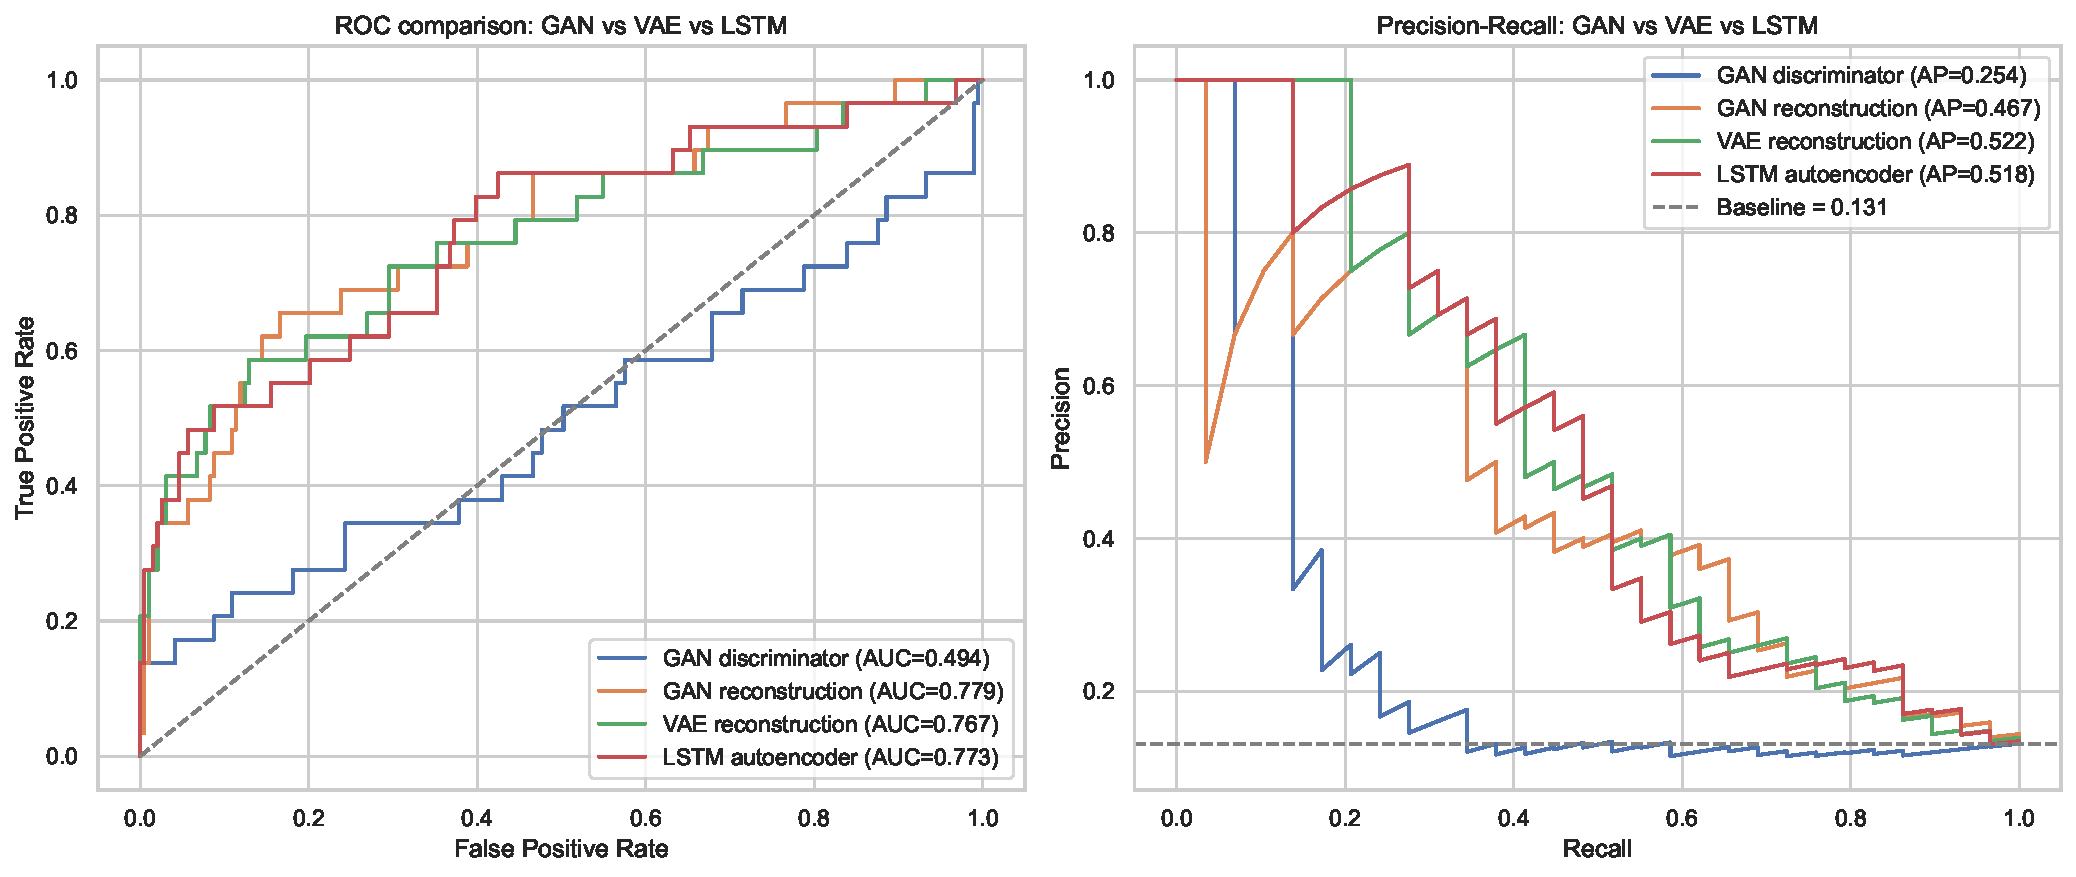
\includegraphics[width=\textwidth,height=0.72\textheight,keepaspectratio]{figures/10_roc_pr_model_comparison.pdf}
		\column{0.36\textwidth}
		\small
		Under the no-leakage split the three reconstruction detectors
		\textbf{converge}: each catches 8/29 crises at 80\% precision.
		\vspace{0.5em}
		\begin{itemize}
			\item Best PR-AUC: \textbf{VAE 0.52}, LSTM 0.52, GAN-recon 0.47.
			\item GAN \emph{discriminator} alone is weak (ROC-AUC $\approx$ 0.49).
			\item Reconstruction beats realism scoring for novelty.
		\end{itemize}
	\end{columns}
\end{frame}

% =========================================================================
\begin{frame}{Does the structure actually separate?}
	\begin{columns}[T,onlytextwidth]
		\column{0.7\textwidth}
		\centering
		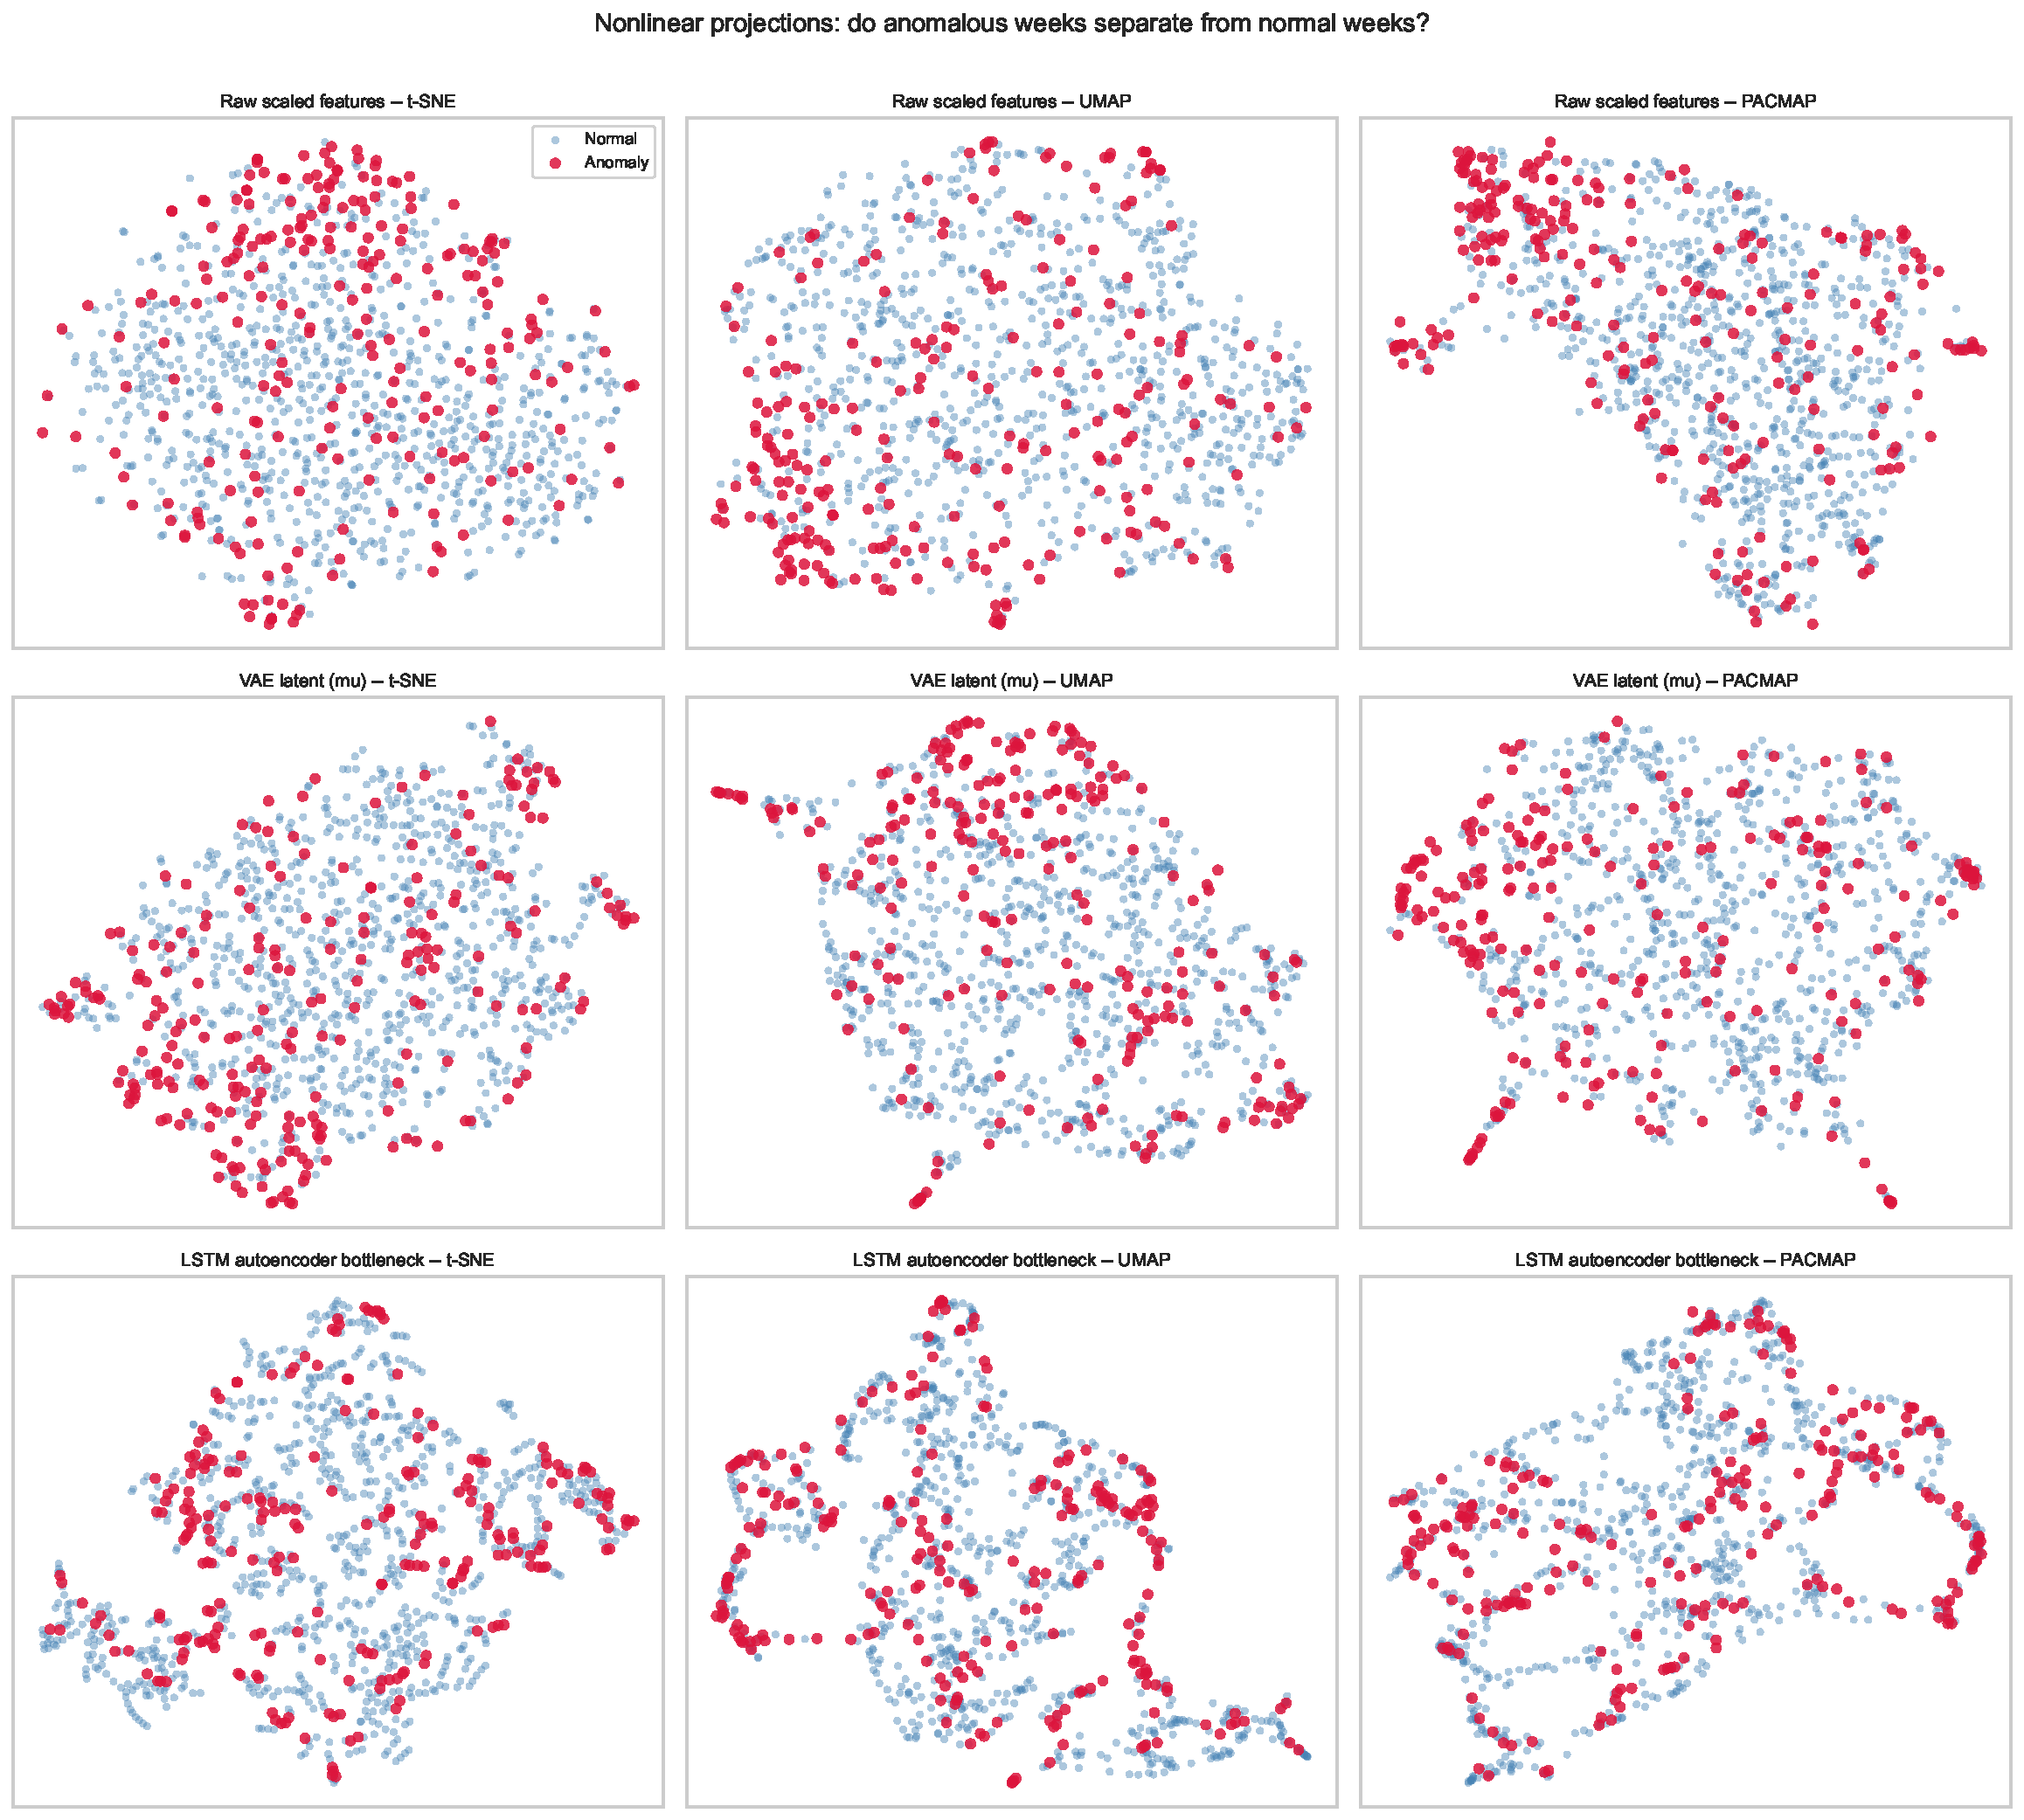
\includegraphics[width=\textwidth,height=0.78\textheight,keepaspectratio]{figures/14_latent_space_dim_reduction.pdf}
		\column{0.28\textwidth}
		\small t-SNE / UMAP / PACMAP on three representations:
		\vspace{0.4em}
		\begin{itemize}\scriptsize
			\item \textbf{Raw features} -- partial separation only.
			\item \textbf{VAE latent} -- barely better.
			\item \textcolor{accent}{\textbf{LSTM bottleneck}} -- clearest cluster; temporal context helps.
		\end{itemize}
		\vspace{0.4em}
		\scriptsize Visual proof that adding short-term context sharpens the manifold.
	\end{columns}
\end{frame}

% =========================================================================
\begin{frame}{Portfolio impact: every flag cuts drawdown}
	\centering
	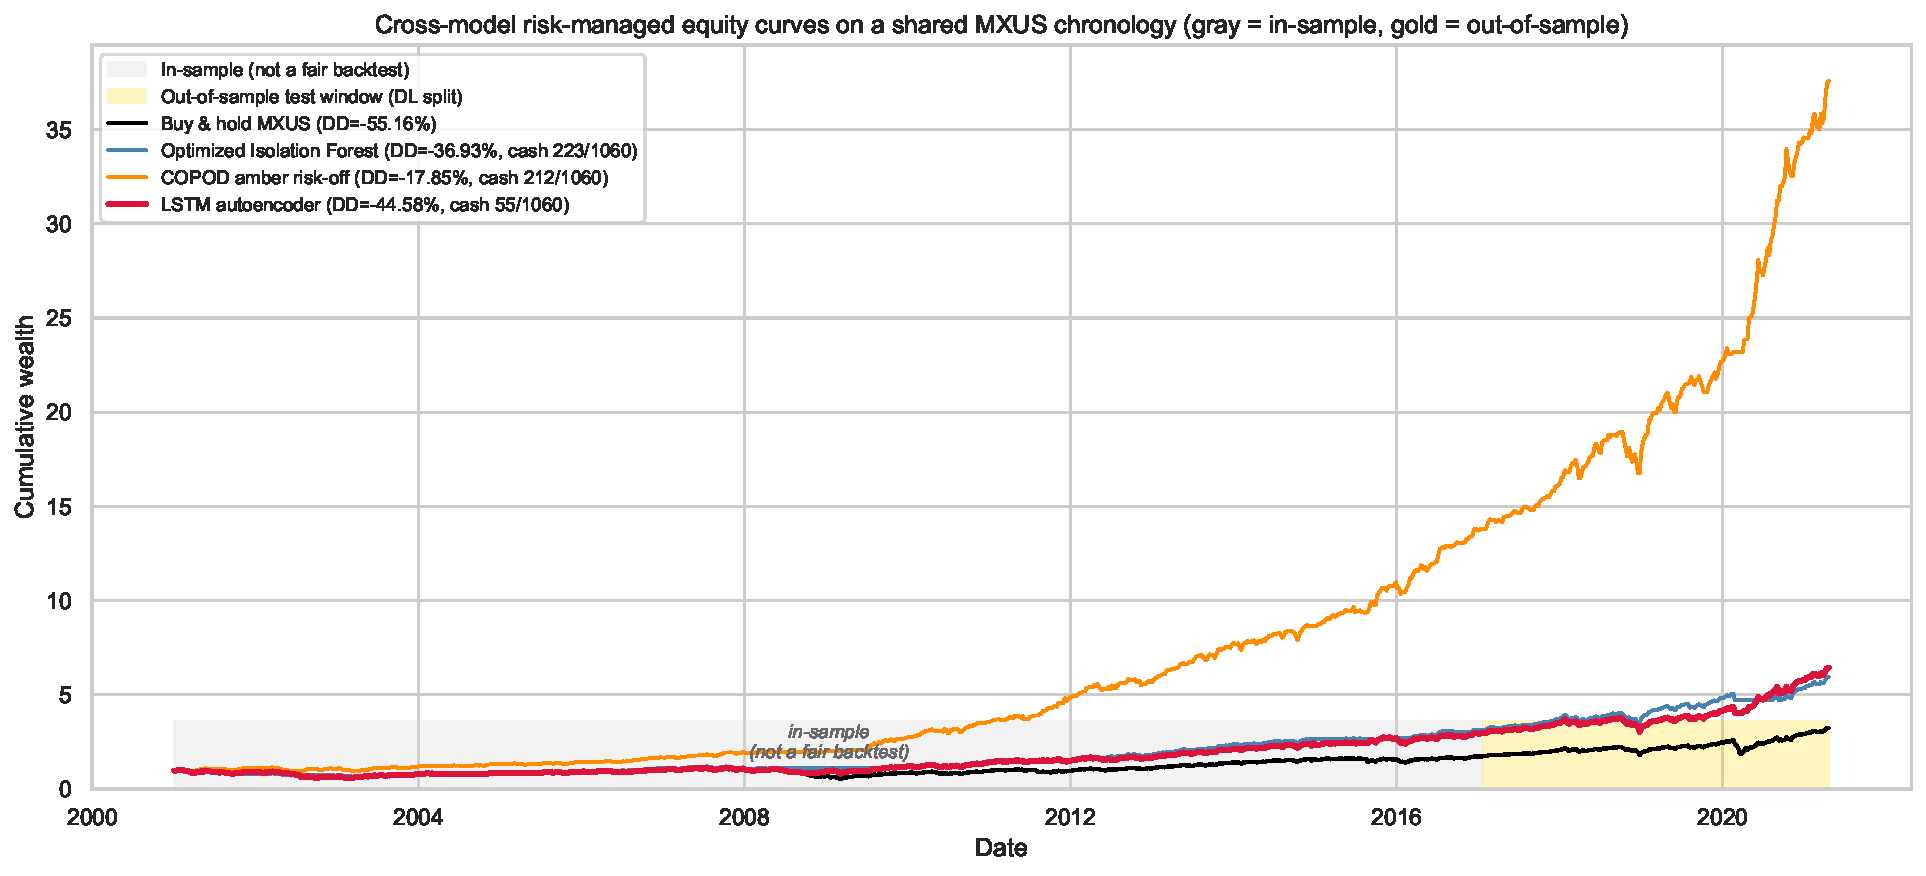
\includegraphics[width=0.74\textwidth,height=0.46\textheight,keepaspectratio]{figures/14_cross_model_equity_curve_comparison.pdf}

	\vfill
	\begin{columns}[c,onlytextwidth]
		\column{0.47\textwidth}
		\textbf{Test-window backtest}\\
		{\scriptsize cash when flagged, else MXUS}
		\vspace{0.2em}

		\scriptsize
		\setlength{\tabcolsep}{5pt}
		\begin{tabular}{lrr}
			\toprule
			Strategy           & Wealth        & Max DD           \\
			\midrule
			Buy \& hold MXUS   & 1.87          & -27.7\%          \\
			LSTM autoencoder   & \textbf{2.03} & -20.2\%          \\
			Optimized IF       & 1.57          & -19.7\%          \\
			COPOD amber        & 1.80          & \textbf{-18.4\%} \\
			\bottomrule
		\end{tabular}

		\vspace{0.3em}
		{\scriptsize Signal acts with a 1-week lag (no same-week look-ahead).}

		\column{0.49\textwidth}
		\footnotesize
		\begin{itemize}
			\item All three \textbf{cut drawdown} vs buy \& hold ($-$27.7\% $\to$ $-$18 to $-$20\%).
			\item \textbf{Only the LSTM also grows wealth} above buy \& hold; IF/COPOD trade
			      return for deeper drawdown control.
		\end{itemize}
	\end{columns}
	\vfill
\end{frame}

% =========================================================================
\begin{frame}{Takeaways}
	\metriccard{Crises caught}{24/29}{Top-$K$ Isolation Forest}
	\hfill
	\metriccard{Best precision}{80\%}{VAE / LSTM / GAN-recon}
	\hfill
	\metriccard{Beats B\&H wealth}{2.03}{LSTM autoencoder}
	\hfill
	\metriccard{Min.\ drawdown}{$-$18.4\%}{COPOD, vs.\ $-$27.7\% B\&H}

	\vspace{0.8em}
	\begin{itemize}
		\item \textbf{A strict chronological split} kills look-ahead bias -- the numbers
		      are conservative but deployable.
		\item \textbf{No single winner}: pick the detector by mandate.
		      Capital preservation $\to$ high-recall Top-$K$ IF; avoid false alarms
		      $\to$ high-precision deep models; balanced $\to$ COPOD.
		\item \textbf{The robust result}: \emph{every} warning system reduces out-of-sample
		      drawdown ($-27.7\%\to-18$ to $-20\%$); the LSTM is the one that also beats
		      buy-and-hold on final wealth.
	\end{itemize}
	\begin{alertblock}{Bottom line}
		Framing market stress as novelty detection turns five very different models into
		one deployable risk-off signal -- and the portfolio drawdown reduction survives an
		honest, leakage-free backtest.
	\end{alertblock}
\end{frame}

\end{document}